En este orden de ideas, es fácil descubrir los primeros términos de la sucesión:\\ $0,1,1,2,3,5,8,13,21,34,55,89,144, \dots$ 

Del mismo modo podemos expresar cada término en base a su función:\\ Fib(0)=0, Fib(1)=1, Fib(2)=1, Fib(3)=2, Fib(4)=3, Fib(5)=5, $\dots$

\subsubsection*{Variante recursiva}

Dada esta definición formal, no es nada difícil crear una primera solución recursiva para obtener un término n de la sucesión de Fibonacci. Pero analicemos a fondo lo que hace esta función. Recursivamente, estará llamando a sus dos anteriores. Cada una de estas llamadas, si es mayor que 1, de nuevo estará llamando a sus dos anteriores. Analicemos el árbol de llamadas para un fibonacci de orden 6:

\begin{figure}[!h]
	\centering
	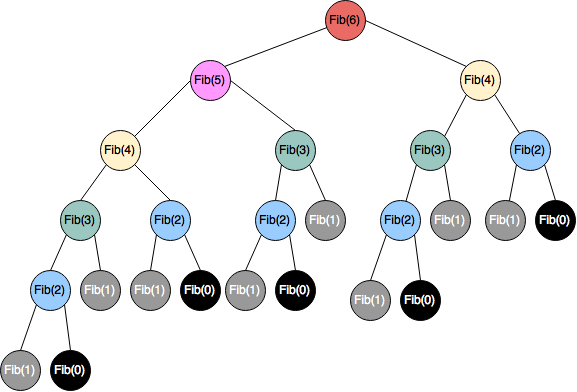
\includegraphics[scale=0.50]{img/arbol-fibonacci.png}
	\label{fig:generalizacion-fibonacci-2}
\end{figure}

Pero es eficiente? Volvamos al árbol. Para calcular 1 vez Fib(6), es necesario calcular 1 vez Fib(5), 2 veces Fib(4), 3 veces Fib(3), 5 veces Fib(2), 8 veces Fib(1) y cinco veces Fib(0) (Como el algoritmo considera constante Fib(1), solo tenemos 5 llamadas a Fib(0). Si Fib(1) se calculara con su antecesor, tendríamos 13 llamadas). ¡Estamos repitiendo operaciones! Y lo peor, estas operaciones se repiten justamente siguiendo la secuencia de Fibonacci como se puede ver en los números en negrilla (1,1,2,3,5,8,13).

\subsubsection*{Variante iterativa}

Si eliminamos los cálculos repetidos, fácilmente podemos tener un algoritmo de iterativo. Para hacer esto, utilizaremos un array que guarde los valores calculados de forma que en la posición $i$  estará la suma de los valores presentes en $i-1$ y $i-2$ partitiendo que para $i$ igual 0 y 1 esos serán sus valores respectivamente. 

Ahora el algoritmo es mucho mas eficiente, reduciendo enormemente el número de operaciones innecesarias para valores altos de $n$. Pero surge un nuevo problema. La complejidad espacial es de $O(n)$ también. Hemos sacrificado espacio por tiempo, ahora tenemos un array de $n$ posiciones cuando en realidad solo necesitábamos la posición $n$ y las demás podemos desecharlas. Como el algoritmo únicamente necesita de los dos valores anteriores para obtener el siguiente podemos remplazar el array por un grupo de tres variables. Ahora la complejidad temporal sigue siendo de orden $O(n)$ pero la complejidad espacial se reduce a un orden $O(1)$.

\subsubsection*{Variante matricial}

Volviendo al inicio, sabemos que:

$Fib(n)=Fib(n-1)+Fib(n-2)$

Partiendo de aquí, podemos fácilmente desarrollar un sistema de ecuaciones:

\[ 0Fib(n-2)+1Fib(n-1)=1Fib(n-1) \]
\[ 1Fib(n-2)+1Fib(n-1)=1Fib(n-1) \]

Y por supuesto, lo reescribiremos en notación matricial:


$
\begin{bmatrix}
	0 & 1 \\ 
	1 & 1
\end{bmatrix}
\begin{bmatrix}
	f(n-2)  \\ 
	f(n-2)
\end{bmatrix}
=
\begin{bmatrix}
	f(n-1)  \\ 
	f(n)
\end{bmatrix} 
$


Verificando estos valores para n = 2


$
\begin{bmatrix}
	0 & 1 \\ 
	1 & 1
\end{bmatrix}
\begin{bmatrix}
	f(0)  \\ 
	f(1)
\end{bmatrix}
=
\begin{bmatrix}
	f(1)  \\ 
	f(2)
\end{bmatrix} 
$


Conociendo que Fib(0)=0 y Fib(1)=1:


$
\begin{bmatrix}
	0 & 1 \\ 
	1 & 1
\end{bmatrix}
\begin{bmatrix}
	0  \\ 
	1
\end{bmatrix}
=
\begin{bmatrix}
	1  \\ 
	1
\end{bmatrix} 
$


Y efectivamente, Fib(2)=1. Ahora bien, generalizando para diferentes valores de $n$.


$
\begin{bmatrix}
	0 & 1 \\ 
	1 & 1
\end{bmatrix}
^{n-1}
\begin{bmatrix}
	0  \\ 
	1
\end{bmatrix}
=
\begin{bmatrix}
	f(n-1) \\ 
	f(n)
\end{bmatrix} 
$

$
\begin{bmatrix}
	0 & 1 \\ 
	1 & 1
\end{bmatrix}
^{n-1}
=
\begin{bmatrix}
	f(n-2) & f(n-1) \\ 
	f(n-1) & f(n)
\end{bmatrix} 
$



Ahora recordemos 3 propiedades de la potenciación:

\begin{enumerate}
	\item $A^{1}=A$
	\item $A^{m^{n}}=A^{mn}$ 
	\item $A^{n}=A^{i}A^{j}$ si $i+j=n$
\end{enumerate}

Los cuales nos permitirán hacer un “divide y vencerás” para resolver la potencia de una manera eficiente.

\begin{figure}[h]
	\centering
	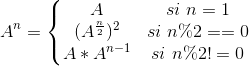
\includegraphics[width=0.3\linewidth]{img/potencias}
	\label{fig:potencias}
\end{figure}

¿Que demonios he hecho? Básicamente, partir el problema. Para explicarlo, miremos paso a paso el proceso para hallar el Fib(11):


\begin{figure}[h]
	\centering
	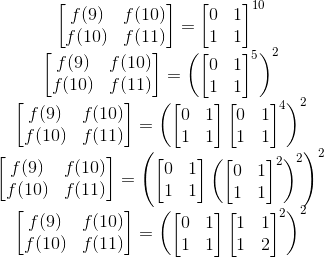
\includegraphics[width=0.3\linewidth]{img/sola}
	\label{fig:solucion3}
\end{figure}

\begin{figure}[h]
	\centering
	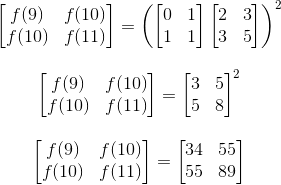
\includegraphics[width=0.3\linewidth]{img/solucion2}
	\label{fig:solucion4}
\end{figure}

Y así llegamos a la respuesta de manera mas rápida.

\subsubsection*{Formula}

Esto no es una última mejora, en realidad es un cambio total. Hasta ahora hemos manejado cada término de la sucesión en base a sus términos anteriores. Pero existe también una formula explicita creada por Lucas para hallar directamente un término sin necesidad de iterar.

$$F_n = \frac{\left(\frac{1 + \sqrt{5}}{2}\right)^n - \left(\frac{1 - \sqrt{5}}{2}\right)^n}{\sqrt{5}}$$

Esta fórmula es fácil de probar por inducción, pero se puede deducir con la ayuda del concepto de funciones generadoras o resolviendo una ecuación funcional.

Puedes notar inmediatamente que el valor absoluto del segundo término siempre es menor que $1$, y también disminuye muy rápidamente (exponencialmente). Por tanto, el valor del primer término por sí solo es casi $F_n$. Esto se puede escribir estrictamente como:

$$F_n = \left[\frac{\left(\frac{1 + \sqrt{5}}{2}\right)^n}{\sqrt{5}}\right]$$

donde los corchetes indican redondeo al número entero más cercano.

Como estas dos fórmulas requerirían una precisión muy alta cuando se trabaja con números fraccionarios, son de poca utilidad en cálculos prácticos.

\subsubsection*{Propiedades de la sucesión de Fibonacci}

\begin{enumerate}
	\item Tan sólo un término de cada tres es par, uno de cada cuatro es múltiplo de 3, uno de cada cinco es múltiplo de 5, etc. Esto se puede generalizar, de forma que la sucesión de Fibonacci es periódica en las congruencias módulo m, para cualquier m.
	
	
	\item Cualquier número natural se puede escribir mediante la suma de un número limitado de términos de la sucesión de Fibonacci, cada uno de ellos distinto a los demás. Por ejemplo, 17=13+3+1, 65=55+8+2.
	
	\item Cada número de Fibonacci es el promedio del término que se encuentra dos posiciones antes y el término que se encuentra una posición después. Es decir:
	
	$ F_{n} = { F_{n-2} + F_{n+1}  \over 2}$
	
	\item Lo anterior también puede expresarse así: calcular el siguiente número a uno dado es 2 veces éste número menos el número 2 posiciones más atrás.
	
	$F_{n+1} = F_{n} * 2 F_{n-2}$
	
	\item El último dígito de cada número se repite periódicamente cada 60 números. Los dos últimos, cada 300; a partir de ahí, se repiten cada $15\times10^{n-1}$ números.
	
	\item La suma de los $n$ primeros números es igual al número que ocupa la posición $n+2$ menos uno. Es decir
	
	$F_{n+2}-1 = F_{n} ... +F_{2}+F_{1}$
	
	\item  La suma de diez números Fibonacci consecutivos es siempre 11 veces superior al séptimo número de la serie.
	
	\item  El máximo común divisor de dos números de Fibonacci es otro número de Fibonacci. Más específicamente
	
	$mcd(F_{n},F_{m}) = F_{mcd(n,m)}$
	
	\item Otras identidades interesantes incluyen las siguientes:
	
	$f_0-f_1+f_2-\cdots+(-1)^nf_n=(-1)^nf_{n-1}-1$
	
	$f_1+f_3+f_5+\cdots+f_{2n-1}=f_{2n}$
	
	$f_0+f_2+f_4+\cdots+f_{2n}=f_{2n+1}-1$
	
	$f_0^2+f_1^2+f_2^2+\cdots+f_n^2=f_nf_{n+1}$
	
	$f_1f_2+f_2f_3+f_3f_4+\cdots+f_{2n-1}f_{2n}=f_{2n}^2$
	
	
	$f_{n+2}^2-f_n^2=f_{2n+2}$
	
	$f_{n+2}^3+f_{n+1}^3-f_n^3=f_{3n+3}$
	
	\item La identidad de Cassini: $F_{n-1} F_{n+1} - F_n^2 = (-1)^n$
	
	\item La regla de la suma: $F_{n+k} = F_k F_{n+1} + F_{k-1} F_n$
	
	\item Aplicando la identidad anterior al caso $k=n$, obtenemos: $F_{2n} = F_n (F_{n+1} + F_{n-1})$
	
	\item De esto podemos demostrar por inducción que para cualquier número entero positivo $k$, $F_{nk}$ es múltiplo de $F_n$.
	
	\item Lo inverso también es cierto: si $F_m$ es múltiplo de $F_n$, entonces $m$ es múltiplo de $n$.
	
	\item Los números de Fibonacci son las peores entradas posibles para el algoritmo euclidiano(Teorema de Lame)
\end{enumerate}

\subsubsection*{Codificación Fibonacci}

Podemos usar la secuencia para codificar números enteros positivos en palabras de código binario. Según el teorema de Zeckendorf, cualquier número natural $n$ se puede representar de forma única como una suma de números de Fibonacci:

$$N = F_{k_1} + F_{k_2} + \ldots + F_{k_r}$$

tal que $k_1 \ge k_2 + 2,\ k_2 \ge k_3 + 2,\ \ldots,\ k_r \ge 2$ (es decir: la representación no puede utilizar dos números de Fibonacci consecutivos).

De ello se deduce que cualquier número puede codificarse de forma única en la codificación de Fibonacci. Y podemos describir esta representación con códigos binarios $d_0 d_1 d_2 \dots d_s 1$, dónde $d_i$ es $1$ si $F_{i+2}$ se utiliza en la representación. El código irá acompañado de un $1$ para indicar el final de la palabra clave. Observe que este es el único caso en el que aparecen dos bits 1 consecutivos. 

$$
\begin{tabular}{cclclcl}
1 &=& 1 &=& $F_2$ &=& $(11)_F$ \\
2 &=& 2 &=& $F_3$ &=& $(011)_F$ \\
6 &=& 5 + 1 &=& $F_5 + F_2$ &=& $(10011)_F$ \\
8 &=& 8 &=& $F_6$ &=& $(000011)_F$ \\
9 &=& 8 + 1 &=& $F_6 + F_2$ &=& $(100011)_F$ \\
19 &=& 13 + 5 + 1 &=& $F_7 + F_5 + F_2$ &=& $(1001011)_F$
\end{tabular}
$$

La codificación de un número entero $n$ se puede hacer con un algoritmo codicioso simple:

\begin{enumerate}
	\item Repita los números de Fibonacci del mayor al menor hasta encontrar uno menor o igual a $n$.
	\item Supongamos que este número fuera $F_i$. Sustraer $F_i$ de $n$ y poner un $1$ en el $i-2$ posición de la palabra de código (indexación desde 0 desde el bit más a la izquierda hasta el más a la derecha).
	\item Repetir hasta que no quede resto.
	\item Añadir una final $1$ a la palabra clave para indicar su final.
\end{enumerate}

Para decodificar una palabra clave, primero elimine la final $1$. Entonces, si el $i$-ésimo bit está configurado (indexado desde 0 desde el bit más a la izquierda hasta el más a la derecha), suma $F_{i+2}$ al número.

\subsubsection*{Módulo de periodicidad p}

Considere el módulo de la secuencia de Fibonacci $p$. Probaremos que la secuencia es periódica.

Demostremos esto por contradicción. Considere el primero $p^2 + 1$ pares de números de Fibonacci tomados módulo $p$:

$$(F_0,\ F_1),\ (F_1,\ F_2),\ \ldots,\ (F_{p^2},\ F_{p^2 + 1})$$

Sólo puede haber $p$ módulo de restos diferentes $p$, y como mucho $p^2$ diferentes pares de restos, por lo que hay al menos dos pares idénticos entre ellos. Esto es suficiente para demostrar que la secuencia es periódica, ya que un número de Fibonacci sólo está determinado por sus dos predecesores. Por lo tanto, si dos pares de números consecutivos se repiten, eso también significaría que los números posteriores al par se repetirán de la misma manera.

Ahora elegimos dos pares de restos idénticos con los índices más pequeños de la secuencia. Deja que los pares sean $(F_a,\ F_{a + 1})$ y $(F_b,\ F_{b + 1})$. Lo demostraremos $a = 0$. Si esto fuera falso, habría dos pares anteriores $(F_{a-1},\ F_a)$ y $(F_{b-1},\ F_b)$, que, según la propiedad de los números de Fibonacci, también sería igual. Sin embargo, esto contradice el hecho de que habíamos elegido pares con los índices más pequeños, completando nuestra prueba de que no existe un preperíodo (es decir, los números son periódicos a partir de $F_0$).